\newcommand{\doctitle}{Construct and Destroy \\ Software Architecture}
\newcommand{\doctitleshort}{C\&D Software Architecture}

\newcommand{\docauthor} {
    \renewcommand{\arraystretch}{0.5}
    \begin{tabular}{l l}
        \textbf{Students:} & ~ \\
        Mark van der Woude     & {\mdseries(S1081655)} \\
        Stephan Schrijver     & {\mdseries(S1078783)} \\
        Jeroen Vinke     & {\mdseries(S1078666)} \\
        Sander Bouwman   & {\mdseries(S1080528)} \\
        Robin T. Koning  & {\mdseries(S1078710)} \\
    \end{tabular}
}

\newcommand{\doctitlepage} {
    \thispagestyle{empty}
    \parbox[t]{1.0\linewidth}{
        \fontsize{40pt}{60pt}\selectfont
        \vspace*{1.5cm}
        \doctitle{}
        \vspace*{1.5cm}
    }
    \vfill
    {
        \centering
        \large
        \hfill \today
        \hfill \docauthor{}
    }
    \normalcolor{}

    \newpage
}

\providecommand{\doctitle}{Title}
\providecommand{\docauthor}{Author}
\providecommand{\doctype}{scrartcl}
\providecommand{\doctitlepage}{TitlePage}

\documentclass[12pt,a4paper,titlepage,parskip=full]{\doctype}

\usepackage[english]{babel}
\usepackage{caption}
\usepackage{float}
\usepackage{blindtext}
\usepackage{hyperref}
\usepackage{graphicx}
\usepackage{listings}
\usepackage{tikz}
\usetikzlibrary{decorations.pathreplacing}
\usepackage{pdfpages}
\usepackage{apacite}
\bibliographystyle{apacite}

% set Listing settings -------------------------------------
\usepackage{listings}
\usepackage{color}

\lstset{frame=tb,
  language=C++,
  backgroundcolor=\color{black!5}, % set backgroundcolor
  aboveskip=3mm,
  belowskip=3mm,
  showstringspaces=false,
  columns=flexible,
  basicstyle={\small\ttfamily},
  numbers=none,
  numberstyle=\tiny\color{gray},
  keywordstyle=\color{blue},
  commentstyle=\color{dkgreen},
  stringstyle=\color{mauve},
  breaklines=true,
  breakatwhitespace=true,
  tabsize=3
}



% Input and output encoding ---------------------------------------------------
\usepackage{iftex}
\ifPDFTeX
   \usepackage[utf8]{inputenc}
   \usepackage[T1]{fontenc}
   \usepackage{lmodern}
\else
   \ifXeTeX
     \usepackage{xltxtra}
   \else
     \usepackage{luatextra}
   \fi
   \defaultfontfeatures{Ligatures=TeX}
\fi

% Math
\usepackage{amsmath}
\usepackage{amsfonts}
\usepackage{amsthm}
\usepackage{amssymb}
\usepackage{mathtools}
\usepackage{bm}
\newcommand{\uvec}[1]{\boldsymbol{\hat{\textbf{#1}}}}

\DeclarePairedDelimiter{\ceil}{\lceil}{\rceil}
\DeclarePairedDelimiter{\floor}{\lfloor}{\rfloor}
\DeclarePairedDelimiter{\bag}{\langle}{\rangle}
\DeclarePairedDelimiter{\set}{\{}{\}}

% Misc
\usepackage{marginnote}
\usepackage[shortlabels]{enumitem}

% Display
\usepackage{lastpage}
\usepackage{fancyhdr}
\setlength{\headheight}{24pt}
\usepackage{eurosym}
\pagestyle{fancy}

\usepackage[nameinlink]{cleveref}

\title{\doctitle}
\author{\docauthor}
\date{\today}

\lhead{\doctitleshort}
\rhead{\today}
\cfoot{\thepage\ /~\pageref{LastPage}}
%\lfoot{\docauthor}

\numberwithin{equation}{section}
\numberwithin{figure}{section}
\numberwithin{table}{section}

\usepackage{changepage}

%Other settings
\lstset{basicstyle=\ttfamily}

\begin{document}
\doctitlepage{}

\tableofcontents
\thispagestyle{empty}
\newpage

\clearpage
\setcounter{page}{1}
\addtocontents{toc}{\protect\thispagestyle{empty}}
\newpage

% Abstract, the intro to our document
\begin{abstract}
\blindtext
\end{abstract}

\newpage

%----------------------------------
% Put new chapters in this block

\section{Selection} In this chapter we will explain how our selection system
works. We will show which classes are involved and how the methods are chained
using UML-diagrams. 

\subsection{User interface} First off, how does the selecting feature works.
You can select a unit by clicking on it using the left mouse button. You can
select multiple by holding the left mouse button and dragging, while dragging a
rectangle is drawn. This rectangle represents the selecting area. When you
release the left mouse button every unit in the selecting area, the red
rectangle, will be selected. A selected unit is recognizable by the red line
around it.

\subsection{Selection process} First we made a handler that handles mouse input
for a panel that represents the world in the user interface. This is the
MouseHandler class, it derives from the SDL\_MouseEventSlot class which derives
from the Slot class. The SDL library provides us with low level access to the
mouse input on the window.  The header file of the MouseHandler can be found 
at \cref{lst:mousehandlerheader}.

\begin{lstlisting}[caption={Mouse handler header file.},
label={lst:mousehandlerheader}]
class MouseHandlerWorld : public SDL_MouseEventSlot {
private: 
    int start_drag_x; 
    int start_drag_y;
    void handle_up(sdl_mouse_event_data data); 
    void handle_down(sdl_mouse_event_data data); 
    void handle(sdl_mouse_event_data);
    void handle_motion(sdl_mouse_event_data);
    void handle_left_button(const vec2 &); 
    void handle_right_button(sdl_mouse_event_data &, const vec2 &);

public: 
    MouseHandlerWorld(); 
    ~MouseHandlerWorld(); 
    void on(sdl_mouse_event_data d) override; 
}; 
\end{lstlisting}

The class has a lot of private methods that handle the different types of mouse
events. It has one method that has been overridden from the base class, which
is the on-method. The on-method is where user inputs comes in. In this method
the input is separated into two groups and will be handled further by other
methods. To make it clear how this works an explanatory activity diagram can be
found at \cref{fig:activitymousehandler} in the appendix to illustrate the
process. 

After the on-method has determined whether the incoming data is a motion event
or button it will be handled further by other methods. We will start with the
motion input.

Motion input is handled by the handle\_motion method. Motion is only
important for us when the user is dragging. This means the user is holding the
left mouse button down while moving the mouse. When the user is dragging we set
the position the mouse has moved to and let the UI component know that the user
is dragging by setting a variable dragging to true. The UI component has two
methods called draw\_selection\_rectangle and render. Whenever the render
method is called and the variable dragging is true it will call the
draw\_selection\_rectangle with the positions set by the last call to the 
handle motion method.

Button input is handled a bit differently since we first need to determine what
kind of event it is and from which button. If the event comes from the right
button, it is an event that will control units. Since that has nothing to do
with this topic we will leave it there and explain it in a different chapter. 

If, however, the event does come from the left button it is to select units. 
When the left button is pressed down we get the position of the cursor. 
This will be the starting position of the selection rectangle. After a button 
down event from the left button, a button up event will inevitably be fired 
from the button. This event means a few things. First off all the user has 
stopped dragging, because we stated earlier that the user is dragging when he's 
holding down the left button. So we set the dragging variable to false. Also we 
reset the positions to be ready for a next drag event. After resetting the 
variables, we call the handle\_up method. This determines whether the event 
was a drag or a click of the left mouse button. A click is when you press and 
release the mouse in the same position or at maximum 10 pixels away from the 
original position. We have implemented it this way so it is easier to click 
moving targets. The handle\_left\_button\_click is called and it selects the 
target on the clicking position, unless there is no target in range.

When you release the left mouse button more than 10 pixels away from the origin
point you are dragging the mouse. The position of the release of the button and
the position of the press will passed to the select\_units\_in\_rectangle
method. The method first calculates the right, left, upper and bottom offsets 
for the rectangle. After this all units inside will be selected by checking 
which of the units that belong to the player are positioned inside the 
rectangle. At \cref{fig:selectiondrag} you can find a picture of a few 
units that are selected by the select\_units\_in\_rectangle function and you 
can also see the red rectangle that has been used to select them. 

\begin{figure}[H] 
    \centering
    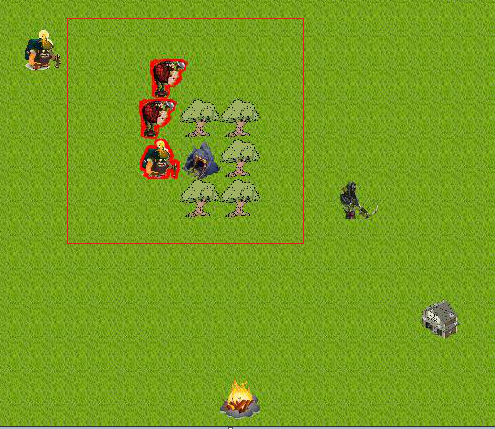
\includegraphics[scale=1.0]{res/SelectionRectangle.png} 
    \caption{Selection by dragging the mouse.}\label{fig:selectiondrag}
\end{figure} 

\newpage

\section{Graph} 
The graph is generated when the game/map is loaded. We’ve decided that our 
graph is a grid-like graph. We start off with generating the nodes, after that 
we generate adjacency edges. A node can have a maximum of 8 edges. When a 
static object is placed we remove edges from the node(s) on which the object 
is placed. We also remove the edges that lead to the node(s) on which the 
object is placed.

There is also a GraphManager which is a Singleton class to avoid making 
multiple graphs. It's also easy to access the graph in different parts of the 
code due to the GraphManager. 

\begin{figure}[H] 
    \centering 
    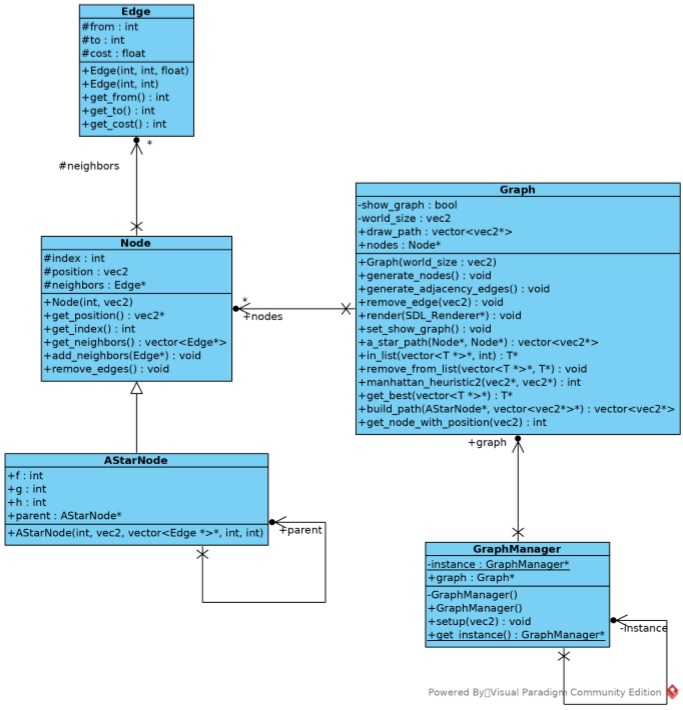
\includegraphics[scale=0.75]{res/graph.jpg}
    \caption{Class diagram for the Graph.}\label{fig:blue-line} 
\end{figure}

\newpage

\subsection{Path Planning}

\begin{tabularx}{\textwidth}{|X|X|}
\hline
\rowcolor{lightgray}\textcolor{white}{\textbf{Test scenario}} &
\textcolor{white}{\textbf{Desired result}}       
\\\hline
An entity plans a new path. &
Entity should plan the most efficient path and must avoid obstacles like buildings.
\\\hline
\rowcolor{lightgray}\textcolor{white}{\textbf{Comments/suggestions}} & 
\textcolor{white}{\textbf{Passed}}
\\\hline
 & \cellcolor{green}                       
\\\hline
\rowcolor{lightgray}\textcolor{white}{\textbf{Tester}} & 
\textcolor{white}{\textbf{Date}}               
\\\hline
Sander Bouwman & May 7, 2017                               		 
\\\hline
\end{tabularx}

\begin{tabularx}{\textwidth}{|X|X|}
\hline
\rowcolor{lightgray}\textcolor{white}{\textbf{Test scenario}} &
\textcolor{white}{\textbf{Desired result}}       
\\\hline
An entity plans a new path to an obstructed area. &
Entity shouldn't do anything because the area can't be reached.
\\\hline
\rowcolor{lightgray}\textcolor{white}{\textbf{Comments/suggestions}} & 
\textcolor{white}{\textbf{Passed}}
\\\hline
 & \cellcolor{green}                       
\\\hline
\rowcolor{lightgray}\textcolor{white}{\textbf{Tester}} & 
\textcolor{white}{\textbf{Date}}               
\\\hline
Sander Bouwman & May 7, 2017                               		 
\\\hline
\end{tabularx}
\newpage

\section{Behaviour}
\label{sec:behaviour}
We've chosen to use the goal driven behavior approach, because entities need to complete different actions to complete a goal. E.g., for a lumberjack to collect wood it needs to plan a path to the resource, then it needs to follow the path, once arrived it should start gathering, etc. Goal driven behavior provides a solid solution for these types of actions. Goals can be very large with loads off sub goals or actions, or they can be very small, this makes goal driven behavior easier extendable compared to state driven behavior for example. Since a goal can consist of multiple smaller goals, the Composite Pattern is a good solution to this problem. You can have small goals such as 'TraverseEdge' and also bigger goals like 'Work' and still treat them the same way. \cite{composite-pattern}

We created a single base class called Goal, which is a template class so that we can reuse it for different entity types. This class, together with the AtomicGoal and CompositeGoal classes, are shown in \cref{fig:goal}. Besides the Goal<T> class, we created two classes that inherit from it, the AtomicGoal and GoalComposite classes. The GoalComposite class contains a deque data structure that contains its subgoals. As you can see in \cref{fig:goal}, the GoalComposite<T> class also contains a couple of extra methods to add, remove, process and remove subgoals.

\subsection{Composite goals}
We created a couple of Composite goals for moving entities which we describe below. There is a class diagram \cref{fig:goalcomposite-inherit} in the appendix that illustrates the structure. This diagram doesn't show all composite goals, however it should give an impressions how we implemented this. 

\subsubsection{Think}
The Think goal is a goal that never gets removed. This goal is needed 
to determine an entity's next goal and activates that goal. It does so by 
calling the goals evaluator class, which returns a desirability value. The 
goal with the highest desirability gets chosen as the next goal. Desirability’s can be influenced by a variant of factors. E.g., how far away is the entity from an hostile entity. When there is an hostile enemy close it might not want to gather resources. Evaluators are a great way to create AI. Instead of using these evaluators we might use fuzzy logic. With fuzzy logic the actions of the entity should even feel more natural. 

\subsubsection{Follow Path}
\label{sec:followpath}
This goal traverses a path by adding the TraverseEdgeGoal class to its 
subgoals. This way a path consists of multiple instances of TraverseEdgeGoals
(\cref{sec:traverseedge}) which can be paused if the entity needs to do 
something else first, i.e. fleeing or resting. Once there are no more edges 
to traverse, this goal will be completed and removed from the entity's 
subgoals.

\subsubsection{Work}
This goal makes the entity go to the nearest resource to work. It first plans 
a path (\cref{sec:planpath}) to the nearest resource and then it follows that 
path (\cref{sec:followpath}). Once it arrives on the resource's location it 
starts to gather the resource (\cref{sec:gatherresource}). Once it's done 
gathering it plans another path, this time to the closest warehouse/depot. It follows 
this path and after it arrives it drops its resources 
(\cref{sec:dropresources}). Once all these goals are completed the work goal is completed as well.



\subsection{Atomic goals}
Besides Composite goals, we also have Atomic goals. You can compare Atomic 
goals with leaf nodes of a tree structure. Atomic goals are the actual actions
 that an entity needs to do. As shown in \cref{fig:atomicgoal-inherit}, an atomic 
 goal has no subgoals. Calling the AtomicGoal::add\_subgoal() method results in an 
 exception.
 
 \begin{figure}[!htb]
    \centering
    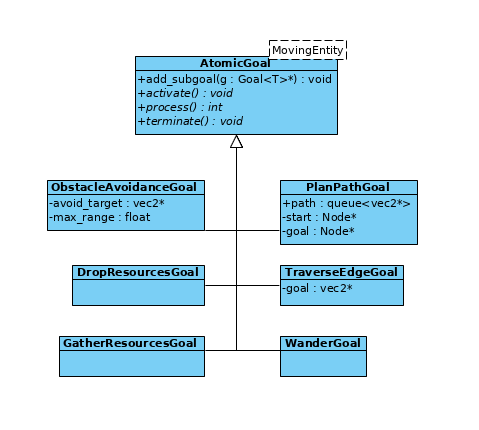
\includegraphics{res/AtomicGoal-Inherit.jpg}
    \caption{AtomicGoal Inheritance.}\label{fig:atomicgoal-inherit}
\end{figure}

\subsubsection{Wander}
The wandering goal is another goal that never gets removed, just like the 
think goal. An entity always needs to wander around if it has absolutely 
nothing to do. The only thing this goal does is activate the wander steering 
behaviour (\cref{sec:wander}).

\subsubsection{Obstacle Avoidance}
The obstacle avoidance goal activates the obstacle avoidance steering 
behaviour. When this goal is activated, it adds the steering behaviour to the 
entity's behaviours. Once the distance to the target that it needs to avoid 
is big enough, the goal is completed and the steering behaviour also gets 
removed from the entity.

\subsubsection{Drop Resources}
\label{sec:dropresources}
Once an entity has gathered enough resources, it needs to drop them at a 
warehouse/depot. This goal simply removes the resources the entity gathered and adds them to the resources of the player. When it dropped all of it's resources at the warehouse, the goal is completed.

\subsubsection{Gather Resource}
\label{sec:gatherresource}
This goal calls the Gather() method from a resource entity. This method extracts resources from the resource entity and adds it to the entity that is gathering the resource. Once the resource entity has been depleted or the maximum carrying capacity of the gathering entity has been reached this goal will be completed.

\subsubsection{Plan Path}
\label{sec:planpath}
The plan path goal plans a path using the A* algorithm, using the Manhattan 
heuristic (\cref{sec:pathplanning}). Once the path has been generated, it gets set as the active path 
for the given entity. This is the only task it needs to complete before 
getting removed from the containing goal.

\subsubsection{Traverse Edge}
\label{sec:traverseedge}
This goal uses the Seek behaviour explained in \cref{sec:seek-behaviour}. Once 
this class gets instantiated it adds an instance of SeekStrategy to the 
entity's behaviour. The only thing it needs to do while processing, is 
to check whether the entity has this behaviour, and if so if it's close 
enough to the next node on the graph. If it's close enough, the goal has been 
completed.


\newpage


\newpage

\section{Controlling workers}

One of the things the player can do is order workers to do a specific task. This is done by selecting one or more workers followed by right clicking somewhere. For example, the player can right click on the ground, which will cause the selected workers to move there. The player can also order workers to gather resources such as wood.

Since the player can select any kind of worker and order it to do many different things, a design pattern was needed to ensure that the code remained readable and extensible. The strategy pattern was chosen because of the fact that it is very extensible. 

A class diagram of relevant classes can be found in \cref{fig:orderstrategies}. The basic idea is that there is one singleton class named MoveOrder with a orderMove function. This function can be used throughout the game to order one or more entities to do something at a certain vector. Based on what the player right clicked on an OrderStrategy is selected. This OrderStrategy takes care of the right click event, for example by ordering the selected entities to go to a certain location.

Down below, in \cref{fig:orderstrategy}, you can find the implementation of the strategy that handles the event where a user orders one or more entities to move to a piece of ground.

\begin{figure}[!htb]
    \centering
    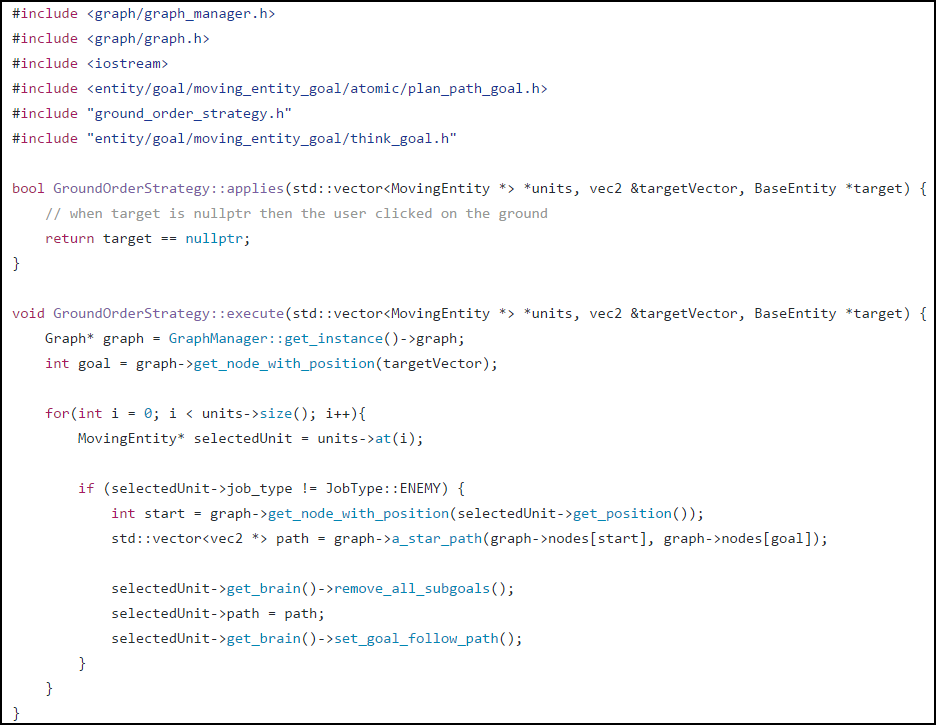
\includegraphics[angle=0,origin=c,scale=0.66]
    {images/order-strategy.PNG}
    \caption{Order strategy}\label{fig:orderstrategy}
\end{figure}


\newpage
%----------------------------------

\bibliography{bib/sources}
\newpage

\section{Appendix}
\begin{figure}[!htb]
    \centering
    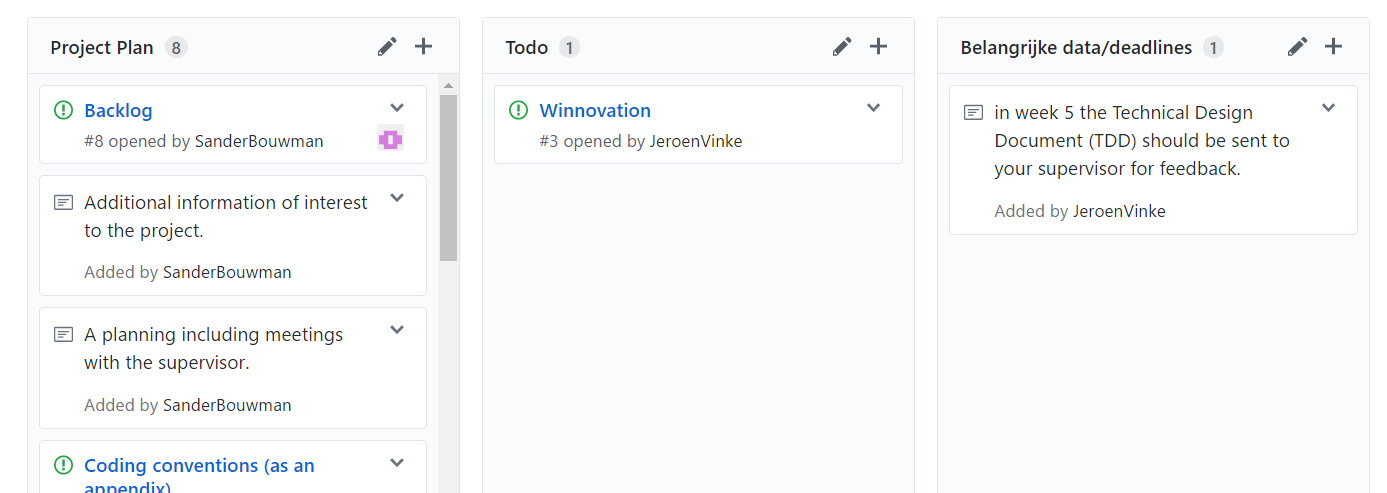
\includegraphics[angle=-90,origin=c,scale=0.75]
    {images/github-projects.PNG}
    \caption{GitHub project}\label{fig:githubproject}
\end{figure}

\end{document}

